
\chapter{Influences de la membrane sur la translocation}
\label{effetsmembrane}

\cleardoublepage

{\Large\textbf{{Effets de la membrane sur la translocation}}}\\

\lettrine[loversize=0.6,lraise=0.1,findent=0.5em,nindent=0em]{D}{}ans ce chapitre, nous décrivons des simulations de translocation à travers une membrane dont les grains sont dans un premier temps plongés dans un potentiel harmonique, ce qui confère des propriétés vibratoires, puis liés entre eux, entrainant de la flexibilité.\\

\minitoc

\newpage

\section{Moyens numériques}

Les résultats que nous avons présenté jusqu'à présent sont le fruit de calculs développés et préparés sur un ordinateur de bureau et réalisés avec l'appoint d'un petit cluster de calcul disponible pour le laboratoire. Dorénavant, nous nous intéressons à des systèmes comportants une membrane non figée, ce qui va augmenter drastiquement les besoins en ressources numériques. En effet, il va maintenant falloir intégrer les équations du mouvement de tous les grains de la membrane et ne plus tenir compte uniquement de leur position.


La partie développement et visualisation avec VMD \cite{HUMP96,STON2001} peut toujours être réalisée avec nos moyens locaux, pour effectuer des tests ponctuels et observer le comportement du système sur quelques trajectoires, mais le gros de la production statistique nécessite des moyens conséquents. Bien que le solveur que nous utilisons, LAMMPS \cite{lammps}, soit efficace et répartisse correctement et de manière homogène l'ensemble des grains sur les processeurs disponibles afin d'optimiser le temps de calcul, le temps de calculs total nécessaire à nos travaux n'en reste pas moins élevé.

Nous avons donc effectué une demande d'allocation de ressources informatiques, dans le cadre de la campagne annuelle DARI \cite{dari} (voir la demande en \hyperref[annexea]{annexe A}) et obtenu 48000 heures de calculs renouvelées une fois, soit 96000 heures de calculs sur le très grand centre de calcul du CEA (TGCC \cite{tgcc}). Cela représente presque 22 ans de calculs ininterrompus si nous avions du nous contenter d'un ordinateur de bureau (11 ans si notre processeur était aussi performants que ceux du tgcc, ou 8 mois en monopolisant entièrement les ressources informatiques de notre petit cluster partagé).

\begin{figure}[H]
\begin{center}
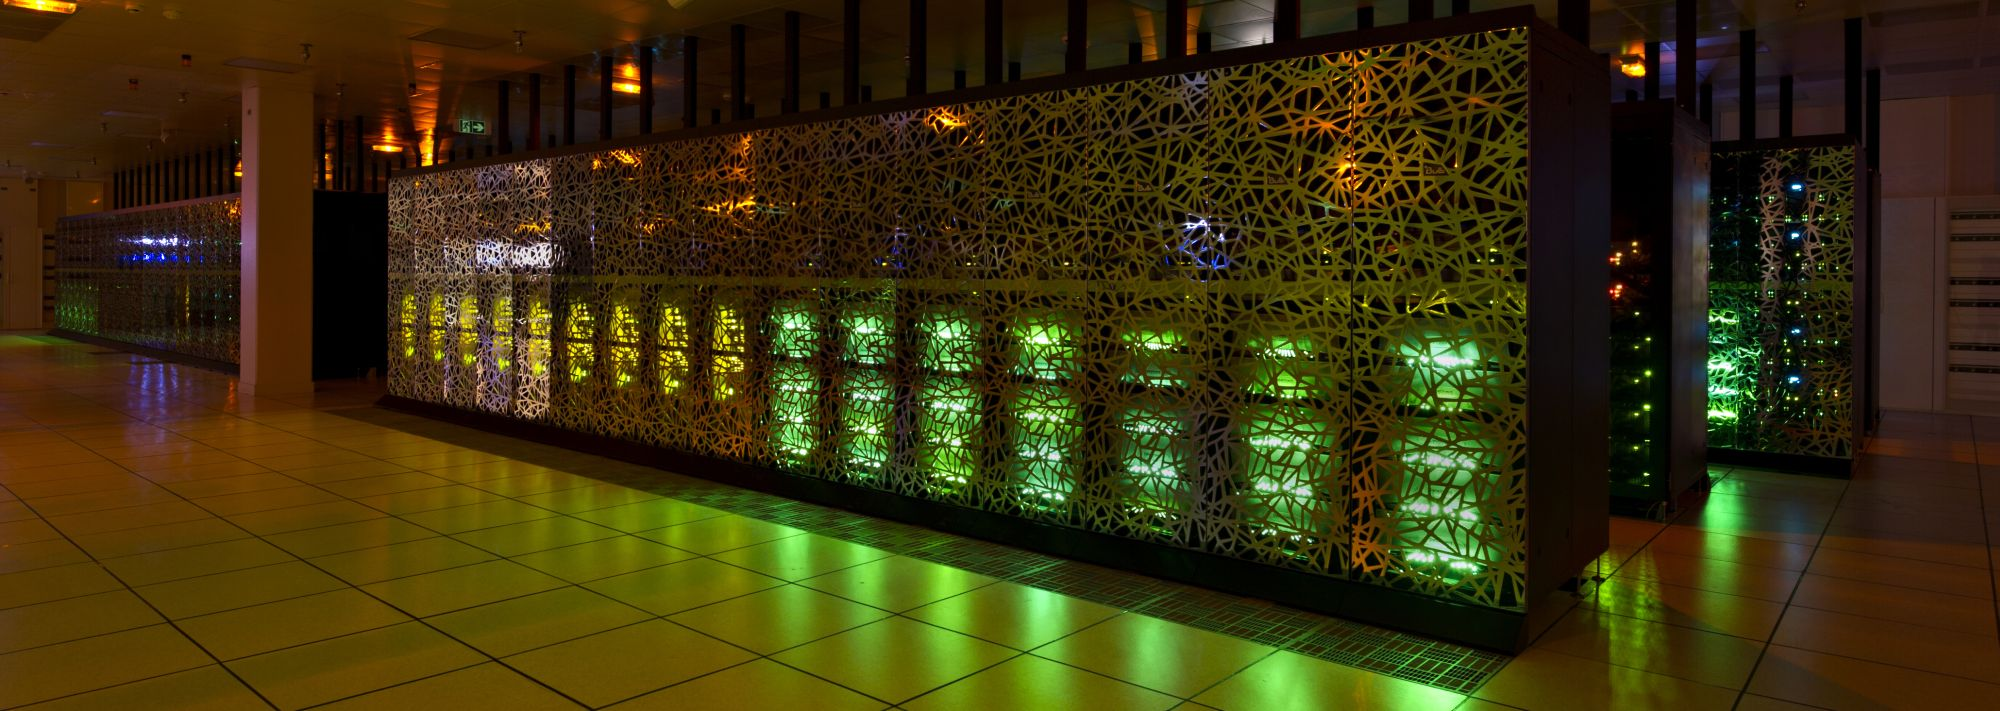
\includegraphics[width=0.8\textwidth]{Curie-M2012_011_Vue_002.jpg}

\caption[TGCC du CEA]{Photo du centre de calcul curie du TGCC du CEA \cite{tgcc}.}
\label{tgcc}
\end{center}
\end{figure}


Une fois les heures allouées, nous avons pu transférer les conditions initiales de nos grains (voir un exemple en \hyperref[annexeb]{annexe B}) et les conditions de simulations pour LAMMPS (exemple en \hyperref[annexec]{annexe C}) au calculateur curie du TGCC (voir figure \ref{tgcc}). Pour limiter l'espace disque utilisé sur le TGCC, nous avons rappatrié régulièrement les données générées sur notre propre matériel en vue d'y effectuer leur post traitement. Ce post traitement a été réalisé principalement en C et en bash (un programme typique pour réaliser l'histogramme de nos distributions est présenté dans l'\hyperref[annexed]{annexe D}). Une fois les données préparées, nous avons réalisé tous les graphes de ce manuscript avec GNUPLOT \cite{gnuplot}.

Ces ressources numériques nous on permis d'aborder les cas d'une membrane vibrante et d'une membrane flexible. Nous présentons les résultats obtenus dans la suite de ce chapitre.



\newpage


\section{Membrane vibrante}
\label{chapitremembvib}

Précédemment, seul la taille $\sigma$ des grains avait une importance dans le cas de la membrane fixe. Dorénavant nous nous interessons à l'effet des vibrations et de la déformabilité du pore sur le temps de translocation. Dans un premier temps, nous placerons donc chacun des grains de notre membrane dans un potentiel harmonique.\\

Ce modèle est proche du cas des membranes fines de graphène \cite{Schneider2010} ou de MoS2 \cite{Feng2015,2Feng2015}, ces dernières étant relativement peu déformables.

Nous reprenons comme base le plan de grains formant un réseau héxagonal que nous avions utilisé dans le cas de la membrane fixe. Cet ensemble de coordonnées est maintenant un ensemble de position d'équilibre $\textbf{r}_n^{0}$ pour nos potentiels dans lesquels seront plongés nos grains constitutifs de la membrane. On a donc pour chaque grain $n$ constituant la membrane un potentiel appliqué de forme quadratique \cite{serway2004physics}:

\begin{center}
\begin{eqnarray}
U_{n}membrane=k(\textbf{r}_n-\textbf{r}_n^{0})^2
\end{eqnarray}
\end{center}
Ceci va nous permettre, comme le montre la figure \ref{2membranes}, d'avoir une membrane présentant des propriétés vibrationnelles.


\begin{figure}[H]
\begin{center}
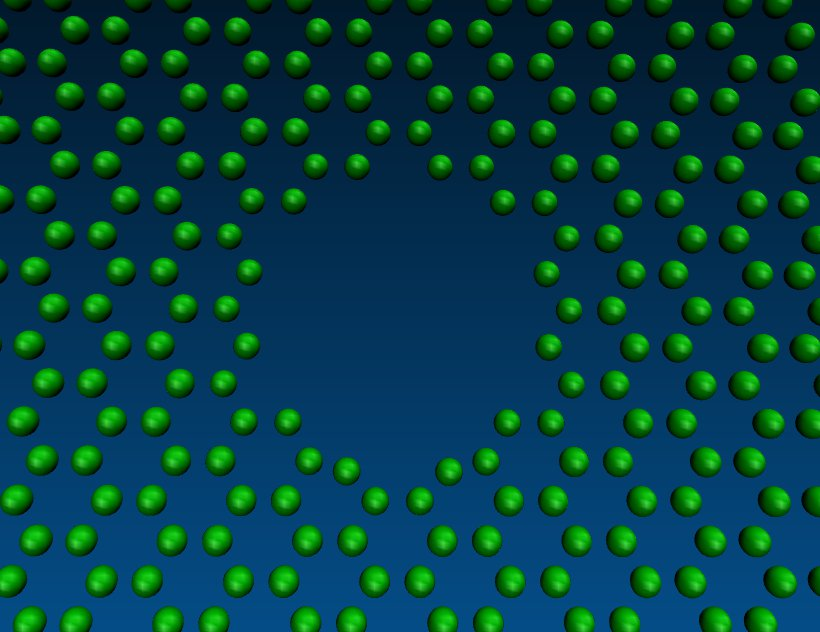
\includegraphics[width=0.45\textwidth]{reseaufix.jpg} \hspace{0.04\textwidth}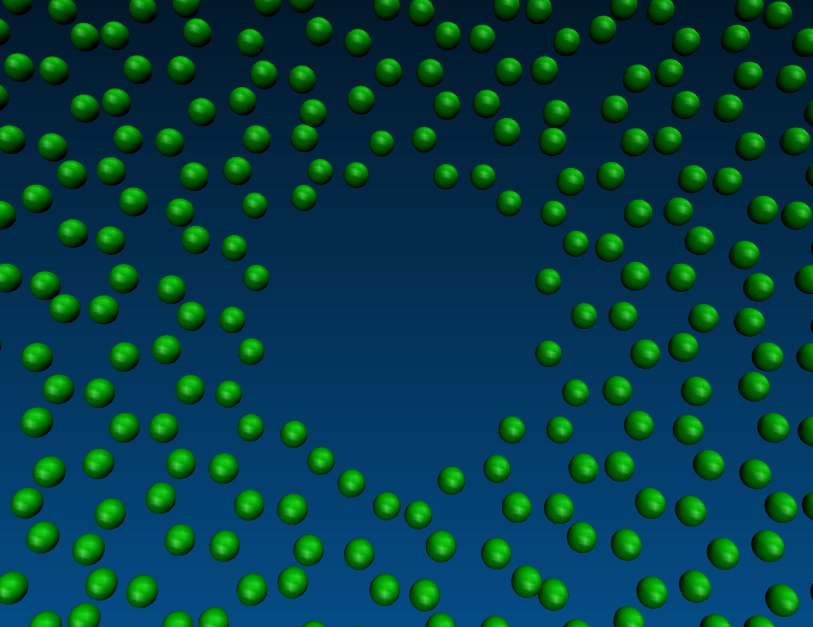
\includegraphics[width=0.45\textwidth]{reseauvib.jpg}

\caption[vibrations de la membrane]{Capture d'écran des membranes lors de la thermalisation. Nous passons d'une membrane fixe (à gauche) à une membrane ayant des propriétés vibrationnelles (à droite).}
\label{2membranes}
\end{center}
\end{figure}

La membrane est définie, en plus de l'ensemble de coordonnées de positions d'équilibre, par la constante de rappel $k$ du potentiel harmonique, mais aussi par la masse $m_n$ des grains, leur coefficient de friction $\nu_n$ avec le solvant et leur température. Nous avons choisi comme base de prendre $m_n=1$, $\nu_n=1$, $k=300$ et $T=1.5$ dans le système d'unité de Lennard-Jones. Cette température de $T=1.5$ correspond à $T_m=T_p$, la température de la membrane et du polymère étant identiques.


\subsection{Taille du pore}



\begin{figure}[H]
\begin{center}
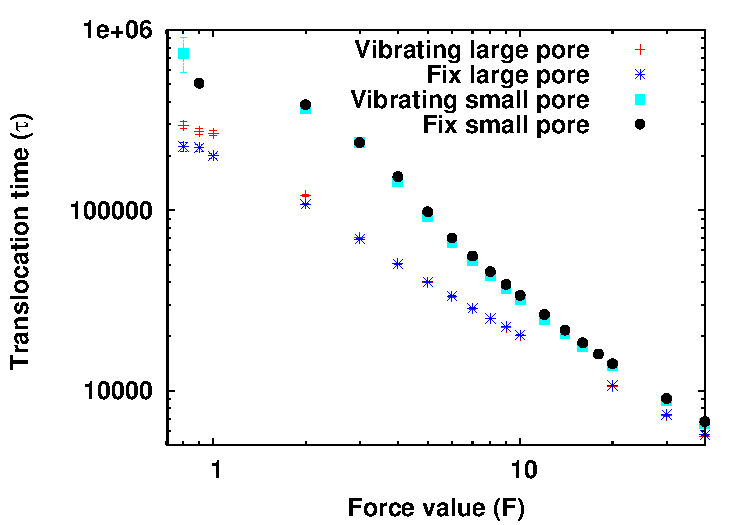
\includegraphics[width=0.9\textwidth]{allforn16.pdf} 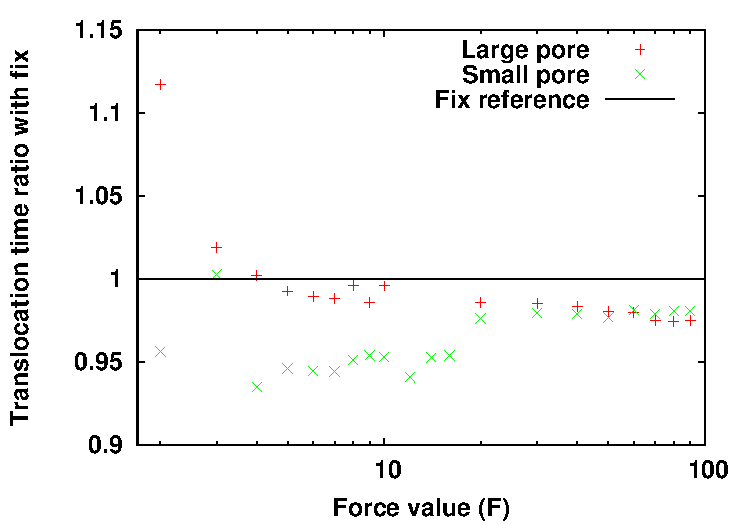
\includegraphics[width=0.9\textwidth]{allforn16comp.pdf}

\caption[Vibrations et taille du pore]{Translocation effectuée avec des vibrations d'une valeur typique. La figure du haut nous montre que la modification du temps de translocation moyen par les vibrations du pore sont très faibles. Sur la figure du bas nous remarquons que les effets sont plus importants dans le cas d'un pore étroit, comme nous nous y attendions. A forte force on ne converge pas vers la référence fixe.}
\label{comptailleporevib}
\end{center}
\end{figure}




\subsection{Convergence entre modèles ?}

La première vérification que nous avons été tenté de faire et d'établir une convergence entre notre membrane fixe précédente et notre membrane vibrante qui devient elle aussi quasi immobile lorsque la valeur $k$ des pièges harmoniques est suffisamment forte. Cependant, comme le montre la figure \ref{convinfforte}, cette convergence n'a pas lieu pour des pièges suffisamment forts pour ne plus être impactés par les effets de la température.


\begin{figure}[H]
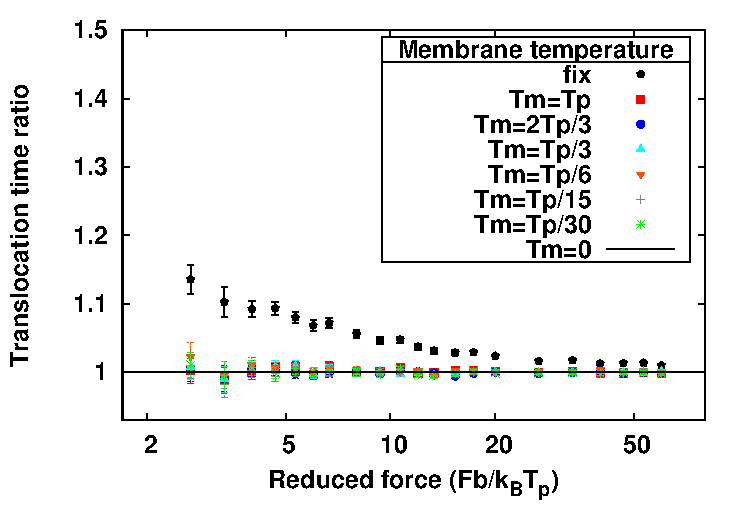
\includegraphics[width=\textwidth]{compkkveryhightonotempkveryhighdifferenttemp.pdf}
\begin{minipage}{0.63\linewidth}
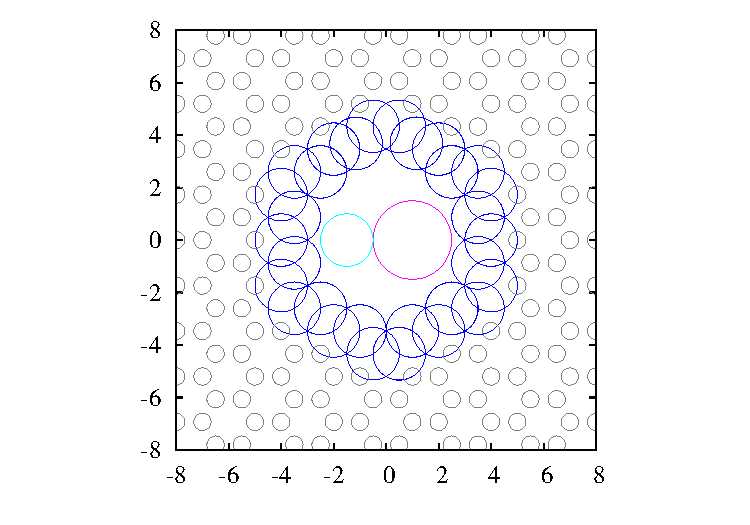
\includegraphics[width=\textwidth]{poreareahighk.pdf}
\end{minipage}
\begin{minipage}{0.37\linewidth} 
\caption[Non convergence des modèles]{Démonstration de la non équivalence entre une membrane fixe et une membrane dont les grains sont plongés dans un piège harmonique fort. Le potentiel est suffisamment fort pour que la température imposée à la membrane n'ai pas d'effets sur la translocation. En effet, les grains de la membrane restent fixes comme le montre la superposition en un unique point pour chaque grain de ses coordonnées au cours de la translocation. Cette non convergence peut s'expliquer par la nature des chocs entre grains qui est modifiée.}
\label{convinfforte}
\end{minipage}
\end{figure}


En effet, précédemment les équations du mouvement n'étaient intégrées que pour les grains constituant le polymère, on avait alors des chocs entre le polymère et la membrane qui étaient parfaitement élastiques. Dans le cas de cette nouvelle membrane, les échanges énergétiques entre membrane polymère sont possibles. Cette dernière affirmation a été testée au cours d'une translocation. Les résultats obtenus (voir figure \ref{temptransloc}) montrent que pendant la translocation (et également pendant la génération de condition initiale), Les atomes du pores peuvent absorber de l'énergie venant du polymère.


\begin{figure}[H]
\begin{center}
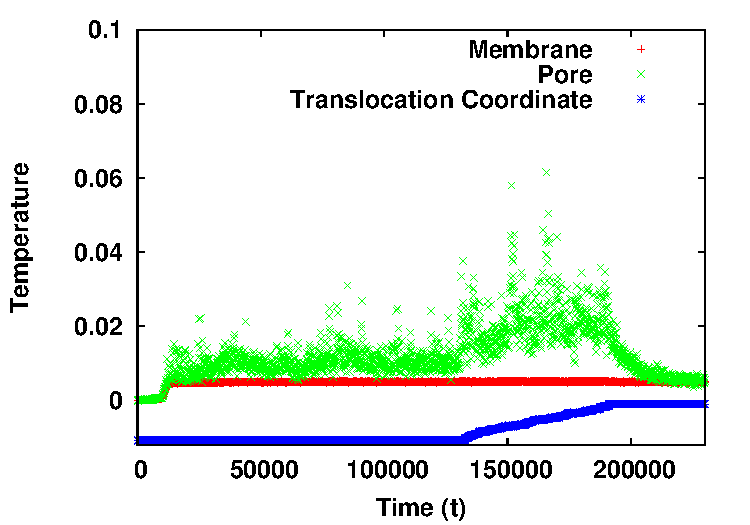
\includegraphics[width=\textwidth]{temptransloc.pdf} 

\caption[Absorption d'énergie par la membrane]{Evolution de la température des grains constituant la membrane au cours de la translocation. La coordonnée de translocation affichée correspond à la valeur réelle a un facteur multiplicatif près afin d'être superposée à l'évolution des températures. La température de la membrane a été choise suffisamment faible pour observer facilement l'apsorption d'énergie.On observe une première phase durant laquelle la memebrane se met à la température imposée. La deuxième phase est lorsque le polymère s'équilibre, les chocs avec le pore augmentent la température de ce dernier. Lorsque la translocation démarre (c'est à dire lorsque la coordonnée de translocation commence a augmenter), on observe une augmentation des contacts et transfers d'énergie. Lorsque la translocation est terminée, la température du pore rejoint celle de la membrane.}
\label{temptransloc}
\end{center}
\end{figure}


\newpage
\subsection{Fréquences vibratoires et suramortissement}

Nous avons recherché dans la littérature des exemples d'influence des propriétés du pore sur le temps de translocation. Le cas le plus proche de ce que nous nous proposons d'étudier concerne des travaux sur l'influence de la fréquence de vibration de la largeur du pore effectués par Cohen et al. \cite{Cohen2011}. Leur travaux sont récapitulés dans la légende de la figure \ref{vibporewidth}.



\begin{figure}[H]
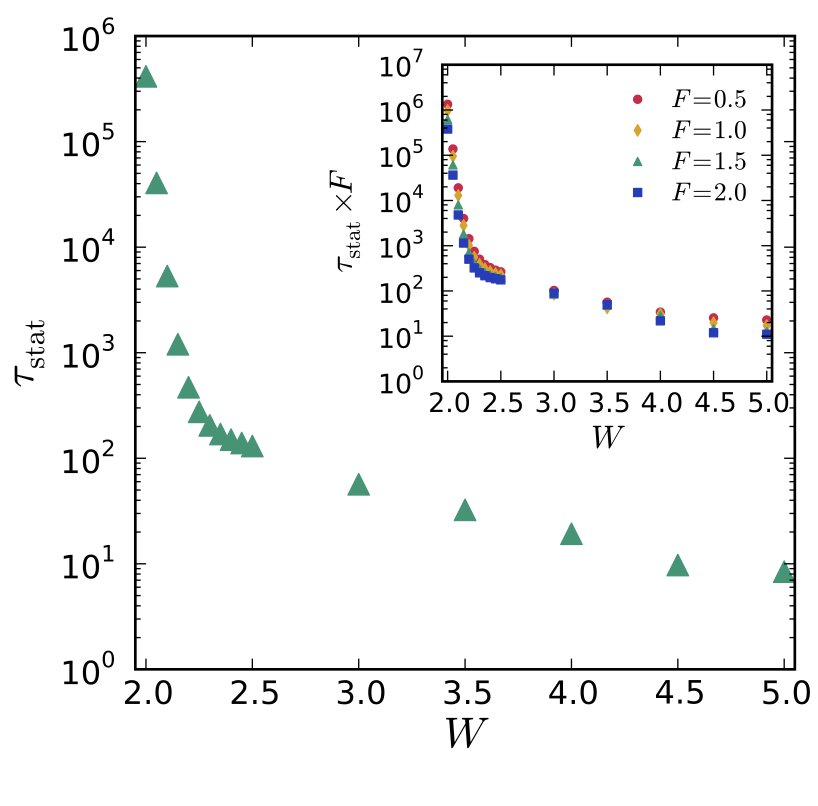
\includegraphics[width=0.5\textwidth]{porevib3.jpg}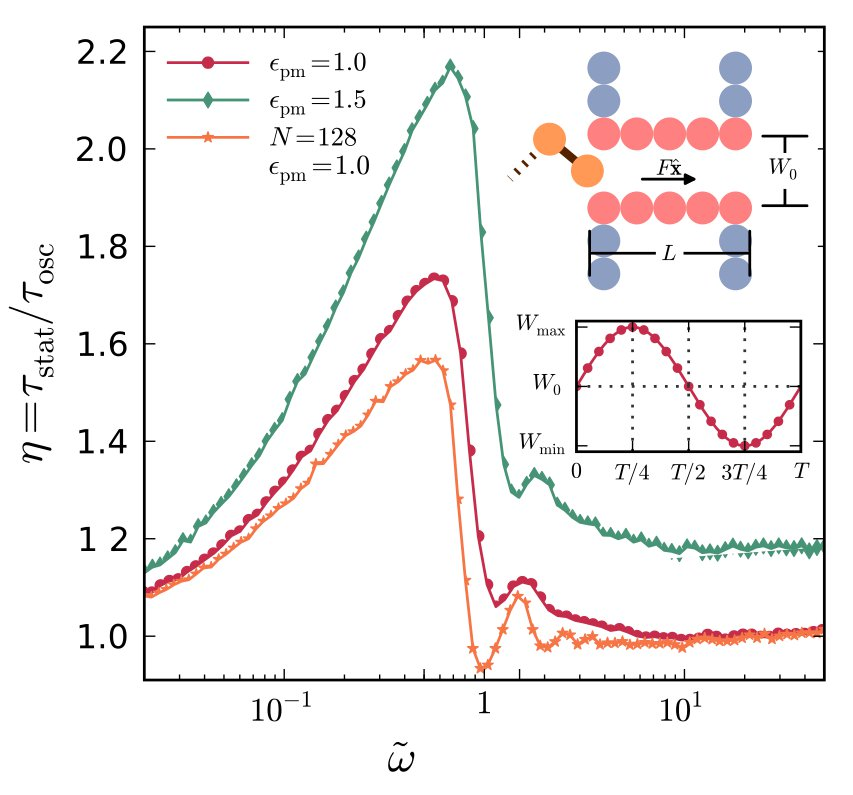
\includegraphics[width=0.5\textwidth]{porevib1.jpg} 
\begin{minipage}{0.5\linewidth}
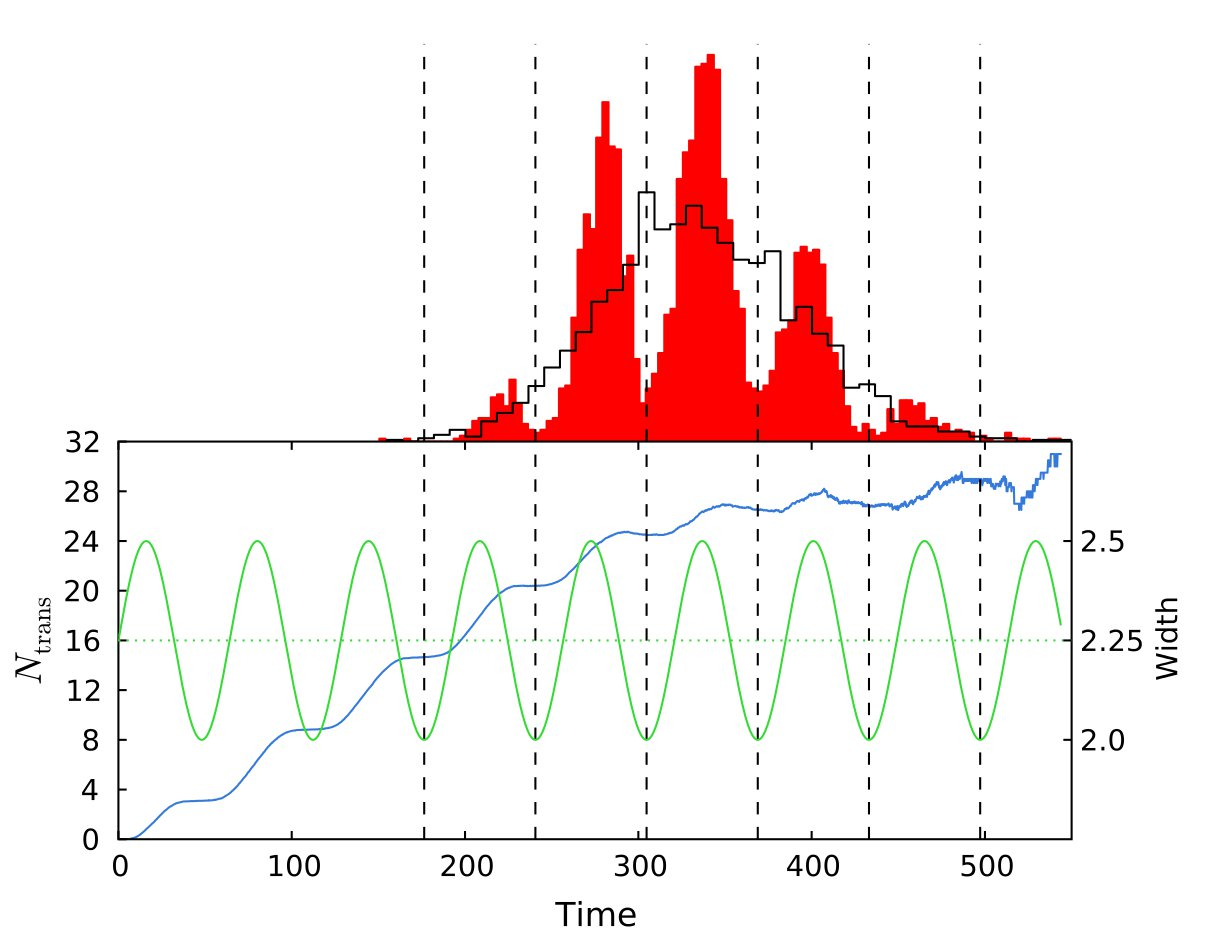
\includegraphics[width=\textwidth]{porevib2.jpg}
\end{minipage}
\begin{minipage}{0.5\linewidth} 
\caption[Vibration imposées]{Travaux réalisés par Cohen et al. \cite{Cohen2011} concernant l'influence de la fréquence de vibration de la largeur d'un nanopore sur le temps de translocation. La figure en haut à gauche démontre, comme nous l'avons également montré dans le \hyperref[sptransloc]{chapitre 3}, que la réduction du diamètre du pore peut significativement augmenter le temps de translocation. La figure en haut à droite démontre que la fréquence imposée à la largeur du pore peut influer sur le temps de translocation, et plus particulièrement sur la distribution des temps comme le montre la dernière figure.}
\label{vibporewidth}
\end{minipage}
\end{figure}

L'oscilation de la largeur du pore de manière sinusoïdale va favoriser ou non le processus de translocation en fonction de la fréquence de ces oscillations. Dans ces travaux, la fréquence de largeur du pore est imposée par l'extérieur. Dans notre cas les vibrations ne peuvent être dues qu'à l'imposition de la température. Nous avons travailé à une fréquence constante (voir figure \ref{influencefrequencecarac}) pour voir s'il était possible d'obtenir des résultats similaires. Nous avons alors une fréquence caractéristique d'oscillation : $\sqrt{\frac{k}{m}}$.







\begin{figure}[H]
\begin{center}
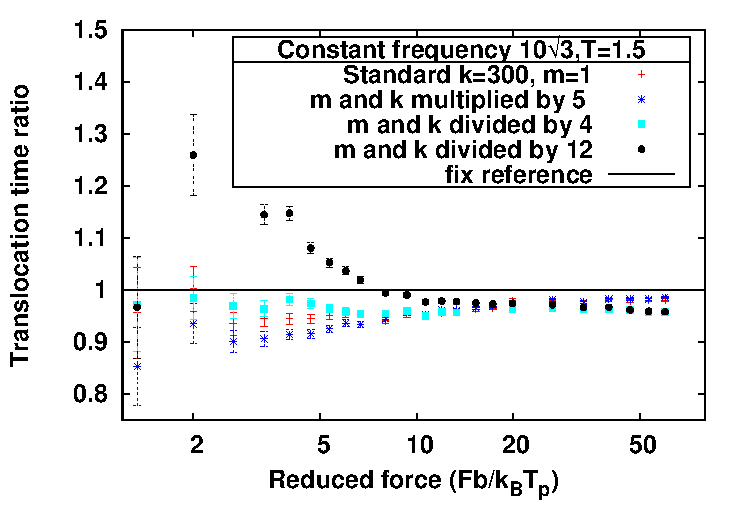
\includegraphics[width=\textwidth]{compsamefrequency.pdf} 

\caption[Influence de la fréquence des vibrations]{Le fait de travailler à fréquence constante ne semble pas garantir un comportement similaire lors de la translocation. L'augmentation des valeurs de $k$ et $m$ semble ralentir la translocation.}
\label{influencefrequencecarac}
\end{center}
\end{figure}

Les résultats obtenus montrent qu'un maintient de la fréquence ne semble pas être lié à un comportement similaire. On observe que l'augmentation de la valeur de $k$ et $m$ entraine une augmentation du temps de translocation. Comment expliquer ces résultats ?

Notre première hypothèse est que, contrairement aux travaux de Cohen et al. \cite{Cohen2011}, nous travaillons avec 3 dimensions et des oscillateurs décorrélés. En effet dans leurs travaux, l'oscillation est imposée extérieurement au système. Dans notre cas, nos oscillateurs sont indépendants. A deux dimensions, il suffit de deux oscillateurs et de connaître leur différence de phase pour définir le pore. Dans notre cas, les oscillations du pores sont du fait de 32 grains décorrélés. Notons, pour cette hypothèse, que Cohen et al. \cite{Cohen2011} observent à forte fréquence un comportement identique au cas d'un pore de taille constante égale à la valeur moyenne de la largeur du pore dont la largeur est sinusoïdale.

La seconde hypothèse est que notre fréquence caractéristique, $\sqrt{\frac{k}{m}}$, soit vide de sens. En effet, lorsque nous regardons les conséquences d'un changement de masse des grains de la membrane sur le temps de translocation, celle ci semblent, comme le montre la figure \ref{influencemasse}, inexistantes. L'explication est que nous nous situons dans le cas d'un régime suramorti, c'est à dire que les termes inertiels de l'équation de Langevin sont négligeables.

\begin{figure}[H]
\begin{center}
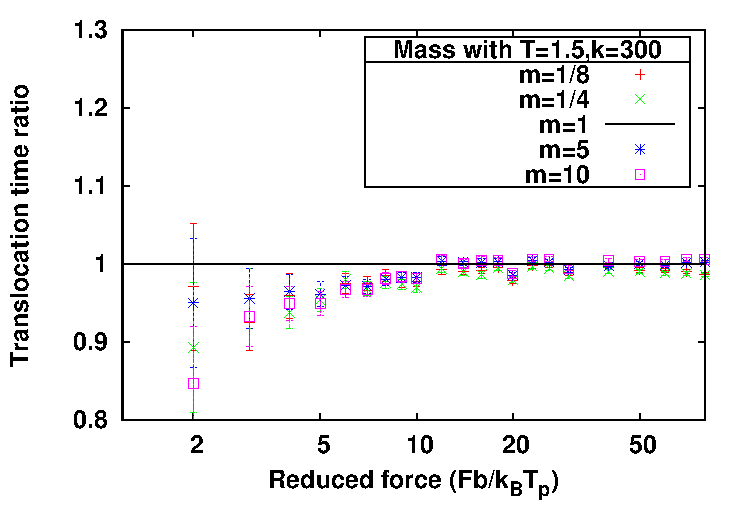
\includegraphics[width=\textwidth]{compmt15.pdf} 

\caption[Influence de la masse]{La masse des grains constituants la membrane ne semble pas avoir d'influence notable sur le temps de translocation. Ceci pourrait être caractéristique d'un régime suramorti.}
\label{influencemasse}
\end{center}
\end{figure}

Cette seconde hypothèse nous semble la plus vraisemblable. En effets, nous utilisons des valeurs de masses comparables à celle des grains du polymère. La bonne adéquation entre les résultats numériques et théoriques, basés sur l'équation de Langevin en négligeant les termes inertiels, dans le cas du polymère, valident a postériori cette hypothèse qui reste ici vraie dans le cas de la membrane.

Si les termes inertiels sont bien négligeables, comme le suggère l'absence d'influence de la fréquence caractéristique et de la masse, notre système n'a plus que trois paramètres, dont seulement deux sont indépendants pour caractériser la membrane (au lieu des quatres dont trois indépendants initialement prévus). Sans termes inertiels, l'équation de Langevin est caractérisée par deux paramètres: $k/\nu$ et $\sqrt{T / \nu}$. Nous avons poursuivi notre étude en conservant le coefficient de frottement $\nu=1$ fixe et en faisant varier la constante des pièges harmoniques $k$ et la température $T$.


\newpage

\subsection{Deux paramètres indépendants}


Afin de décorréler l'influence de nos deux paramètres indépendants, nous avons commencé par étudier l'influence de l'amplitude du piège harmonique lorsque la température de la membrane est nulle, voir figure \ref{influencek}.

\begin{figure}[H]
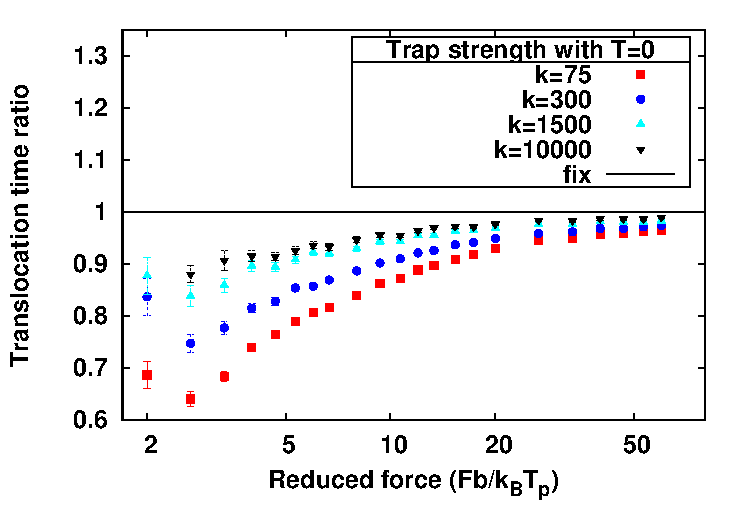
\includegraphics[width=\textwidth]{compkt0.pdf}
\begin{minipage}{0.63\linewidth}
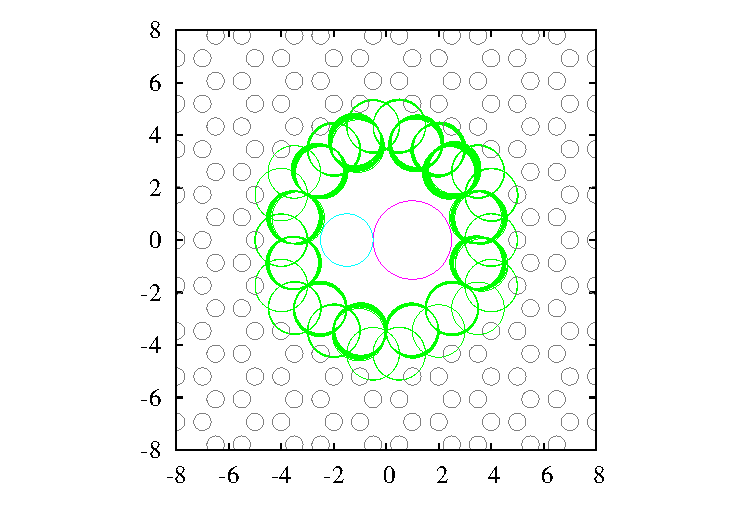
\includegraphics[width=\textwidth]{poreareanotempknorm.pdf}
\end{minipage}
\begin{minipage}{0.37\linewidth} 
\caption[Influence de l'amplitude du piège harmonique]{Lorsque la température de la membrane est nulle, plus l'amplitude du piège harmonique est faible, plus le pore est déformable et la translocation facilitée. En effet, pour de faibles valeurs de $k$, la surimpression des coordonnées des grains au cours de la translocation montre que les grains les plus proches du centre du pore peuvent être déplacés selon l'axe reliant le grain au centre, lors de chocs avec le polymère.}
\label{influencek}
\end{minipage}
\end{figure}

Cette étude permet de montrer qu'une faible valeur de $k$ facilite la déformation du pore à température nulle et donc diminue le temps de translocation. Il reste donc a déterminer l'influence de la température.

\newpage

Afin d'oberver une certaine influence de la température, nous allons devoir nous placer dans un cas ou la valeur de $k$ n'est pas trop élevée, car sinon, comme le montre la figure \ref{convinfforte}, aucun effet notable ne pourra être observé. Nous avons donc opté pour la valeur standart de $k=300$ et reportons les résultats obtenus sur la figure \ref{influencetemperature}.


\begin{figure}[H]
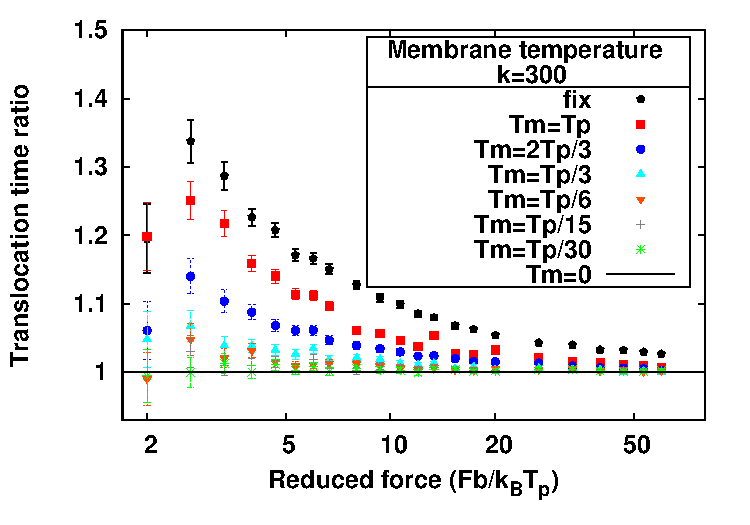
\includegraphics[width=\textwidth]{compkstandarttonotempdifferenttemp.pdf} 
\begin{minipage}{0.63\linewidth}
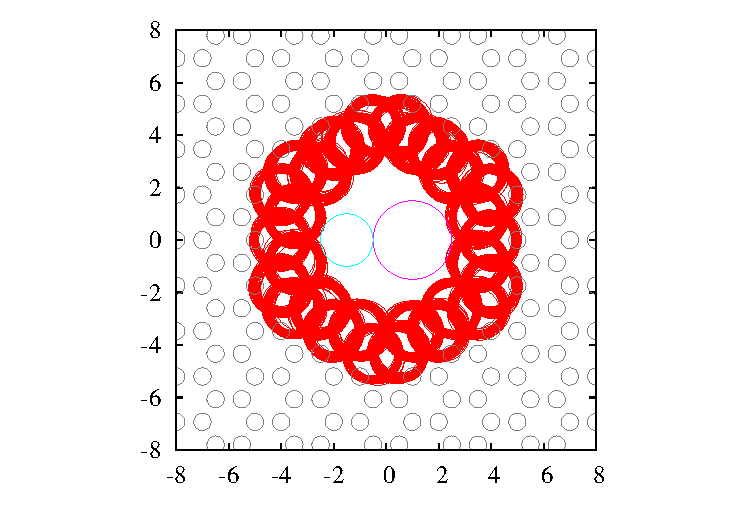
\includegraphics[width=\textwidth]{poreareawtempknorm.pdf}
\end{minipage}
\begin{minipage}{0.37\linewidth} 
\caption[Influence de la température]{Pour une valeur de $k$ donnée, l'augmentation de la température augmente l'amplitude des vibrations. Ces vibrations réduisents l'ouverture effective du pore, comme le suggére la surimpression des positions des grains du pore au cours de la translocation, et ralentissent donc la translocation.}
\label{influencetemperature}
\end{minipage}
\end{figure}

 Nos résultats laissent penser que l'augmentation de la température semble augmenter l'amplitude des oscillations qui réduisent la taille effective du pore et ralentissent la translocation.
 \newpage
 
 Nous avons donc deux effets antagonistes, accélération de la translocation par la déformabilité du pore et ralentissement à cause des vibrations d'origine thermique de la membrane. L'un est il plus important que l'autre ? La figure \ref{antagonismesinfluence} montre qu'ils sont d'ordre de grandeur semblable et l'augmentation de la température permet de passer de la prépondérence d'un effet à l'autre.

\begin{figure}[H]
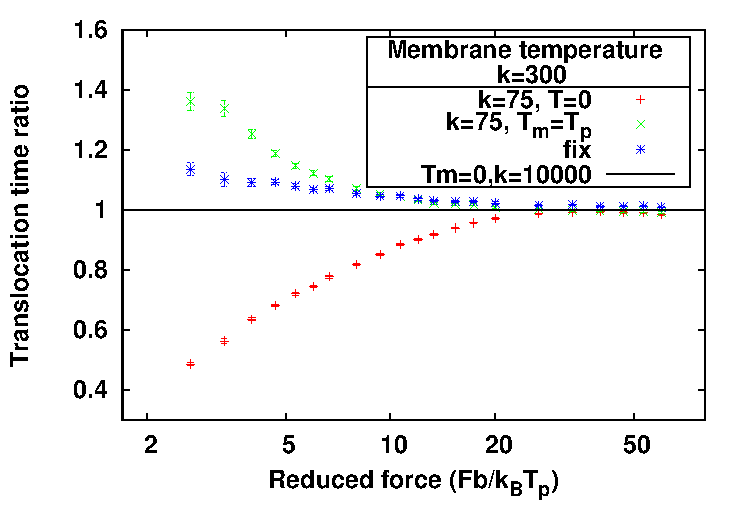
\includegraphics[width=\textwidth]{compbothbehaviour.pdf} 
\begin{minipage}{0.63\linewidth}
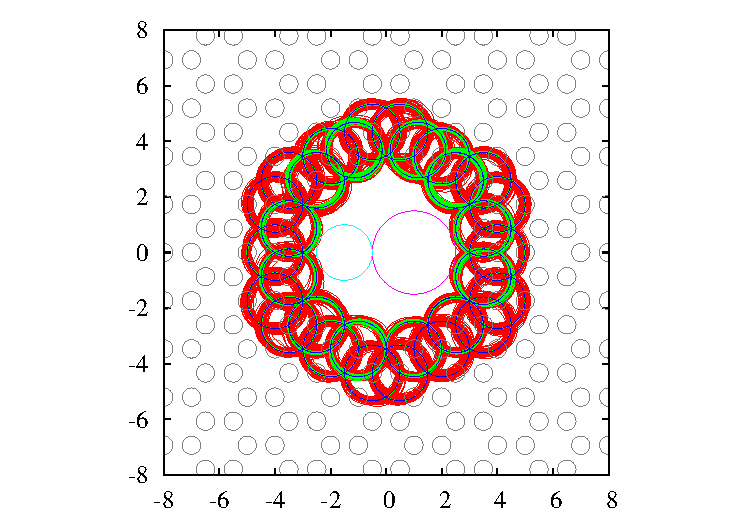
\includegraphics[width=\textwidth]{poreareaall.pdf}
\end{minipage}
\begin{minipage}{0.37\linewidth} 
\caption[Antagonisme des effets observés]{Les deux tendances observées sont dues à des effets antagonistes. Pour une valeur de $k$ faible, on peut avoir une forte déformabilité qui favorise la translocation, mais à partir d'une certaine température, l'effet des vibrations surpasse celui de la déformabilité. La surimpression des trois trajectoires étudiées permet de visualiser le comportement du pore au cours de la translocation.}
\label{antagonismesinfluence}
\end{minipage}
\end{figure}

Nous avons donc montré que pour une valeur de $k$ donnée, une température nulle augmente la vitesse de translocation en permettant la déformabilité du pore, ce processus est concurrencé, lors de la prise en compte de la température, par une réduction de la vitesse due aux vibrations du pore qui réduisent sa taille effective. Il est intéressant de noter que les vibrations et déformations n'ont pas de direction priviliégiée comme le montre le tracé à trois dimensions de la figure précédente \ref{3dplotpore}.


\begin{figure}[H]
\begin{center}


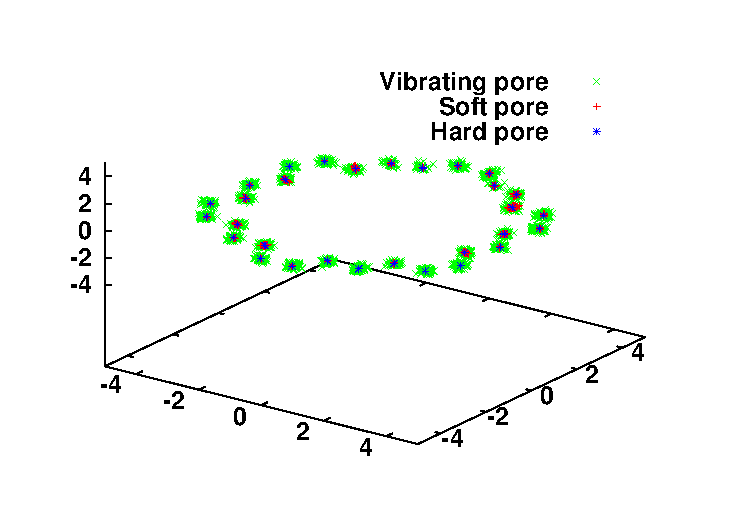
\includegraphics[width=1\textwidth]{porearea3d.pdf} 

\caption[Déplacement du pore à trois dimensions]{Vibrations du pore tracées à trois dimensions. Il n'y a pas de direction de vibration et/ou de déformation privilégiée dans le cas de la membrane dont les grains sont plongés dans des potentiels harmonique.}
\label{3dplotpore}
\end{center}
\end{figure}

\newpage

Nous nous sommes demandés s'il était possible de réduire les effets de la température a une réduction du pore à la taille effective de ce dernier du aux vibrations. Nous avons donc effectué une simulation à température nulle avec une valeur d'intréraction stérique, $\sigma$, de la membrane légérement plus élevée pour que la taille des grains de la membrane soit telle que le pore soit réduit de l'ordre de grandeur de la racine du déplacement carré moyen du cas précédent lorsqu'il y avait des vibrations d'origines thermique.
 
Les résultats obtenus présentés sur la figure \ref{reducedpore}, montrent que le cas est un peu plus compliqué et que bien qu'allant dans le même sens, les effets obtenus dans les deux cas ne sont pas exactement de même amplitude. Il semblerait que nous ayons trop réduit le pore en considérant la racine du déplacement carré moyen.


\begin{figure}[H]
\begin{center}
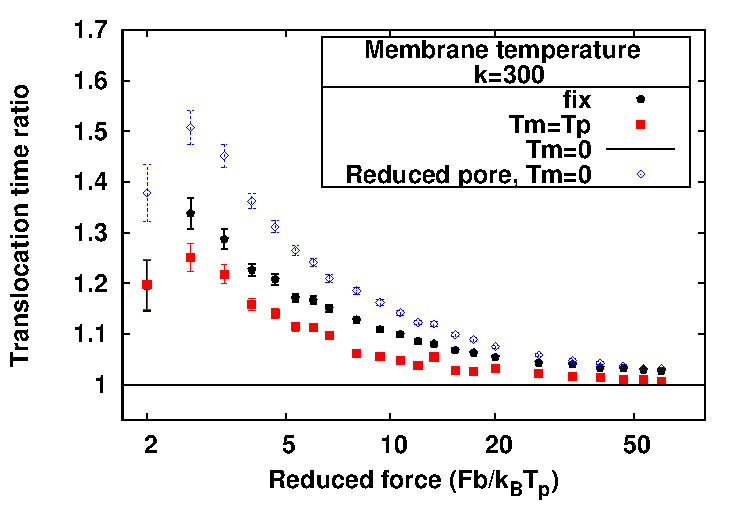
\includegraphics[width=\textwidth]{compkstandarttonotempdifferenttempnew.pdf} 

\caption[Equivalence entre vibrations et pore réduit ?]{Bien qu'allant dans le même sens, la réduction du pore de l'ordre de grandeur du déplacement carré moyen engendré par les vibrations est plus contraignante que les seules vibrations. La surface effective du pore est surestimé en prenant en compte le déplacement carré moyen.}
\label{reducedpore}
\end{center}
\end{figure}

Bien que mal évaluée, l'idée d'une réduction de la surface effective du pore par les vibrations d'origines thermique nous semble pertinente.\\

Intéressons nous maintenant au cas d'une membrane qui en plus d'être déformable et de présenter des propriétés vibrationnelles peut dorénavant se déformer dans son ensemble.





\newpage




\section{Membrane flexible}
\subsection{Définition de la membrane}
\label{chapitrememflex}

Nous allons maintenant étudier le cas d'une membrane flexible. Expérimentalement, cela se rapproche plus des membranes fines à base d'origamis d'ADN \cite{2Bell2012,HernndezAinsa2013} que le cas précédent, plus adapté aux membranes constituées de cristaux. Cette fois ci nos grains constituant la membrane ne sont plus plongés dans un potentiel harmonique mais liés entre eux.\\

Le réseau hexagonal ne nous sert plus qu'à donner un ensemble de coordonnées initiales. Afin d'empêcher la dérive de la membrane, deux bords opposés sont maintenus immobiles. Chacun des grains de la membrane est lié à ses plus proches voisins (c'est à dire 3 grains dans le cas général et 2 pour les grains situés sur le contour du pore ou aux extrémités de la membrane).

Nous avons choisi des liaisons de type FENE afin que l'extension maximale des liaisons puisse garantir la structure de notre membrane. Les paramètres indépendants de notre membrane sont donc maintenant : $k$ préfacteur énergétique caratéristique de nos liaisons, $\sigma_m$ et $R_{0m}$ les caractéristiques géométriques de nos liaisons, $T_m$ sa température, $\nu$ le coefficient de friction des grains. 

\begin{figure}[H]
\begin{center}
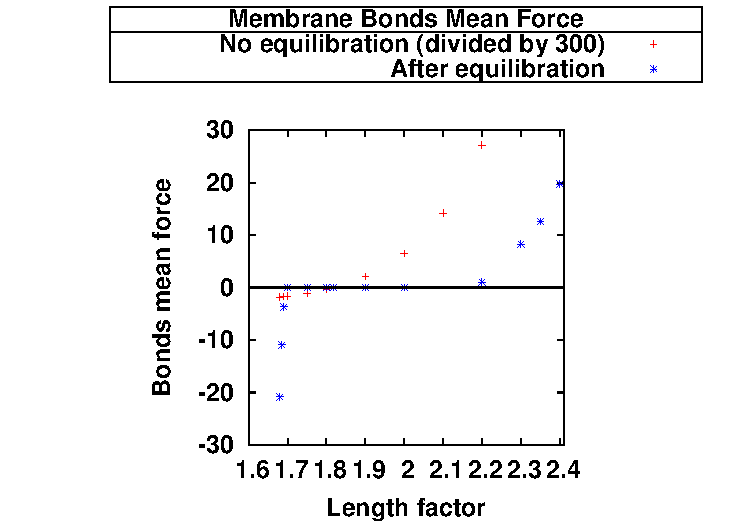
\includegraphics[width=0.9\textwidth]{membranetensionplot.pdf}
\caption[Tension de la membrane]{Après équilibration à température nulle, on observe trois zones. Dans la première zone, la force moyenne des liaisons est négative (donc attractive), la membrane est tendue. On a ensuite un plateau sur lequel la tension est nulle. Puis une troisième zone où les liaisons sont répulsives et la membrane est sous pression. Ne pas permettre au système de s'équilibrer permet de repérer le point de tension nulle qui ne va pas entrainer de déformation de la membrane.}

\label{tensionmembrane}
\end{center}
\end{figure}

Par rapport au cas précédent, les vrais nouveaux paramètres sont les paramètres géométriques de la membrane. Le fait de maintenir deux bords de la membrane impose une dimension donnée pour la membrane.
Les contacts entre membrane et polymère seront régis comme dans le cas précédent par des intéractions de Lennard-Jones avec $\sigma{ij}=1$. Pour la membrane on prendra comme base $\sigma_m= 1/3$ et $R_{0m}=1.5$. Nous multiplions ces valeurs par un unique paramètre géométrique $lf$ (Length factor) pour évaluer la tension de la membrane (voir figure \ref{tensionmembrane}). Le cas de référence utilisé pour comparer les effets des propriétés de la membrane sera celui de la membrane vibrante avec $k$ très grand et $T_m$ nulle, c'est à dire une membrane quasiment fixe avec des échanges énergétiques possibles entre la membrane et le polymère.

La variation de $lf$ permet de distinguer trois régimes de tension repérés sur la figure \ref{tensionmembrane} et illustrés par la figure \ref{snapshottensionmembranesnapshot}. Etudions ces trois cas qui permettent de travailler à taille de membrane constante.

\begin{figure}[H]
\begin{center}
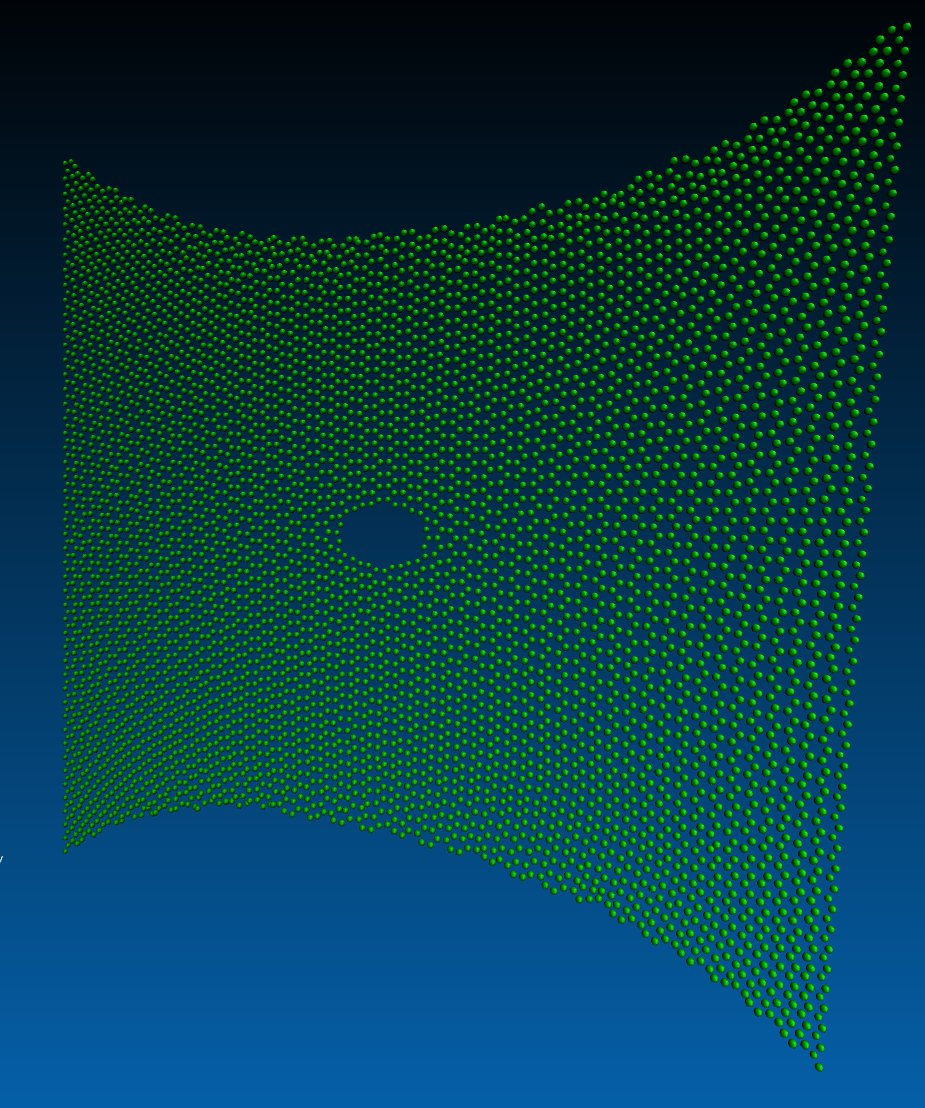
\includegraphics[width=0.5\textwidth]{snapmembranetendue.jpg}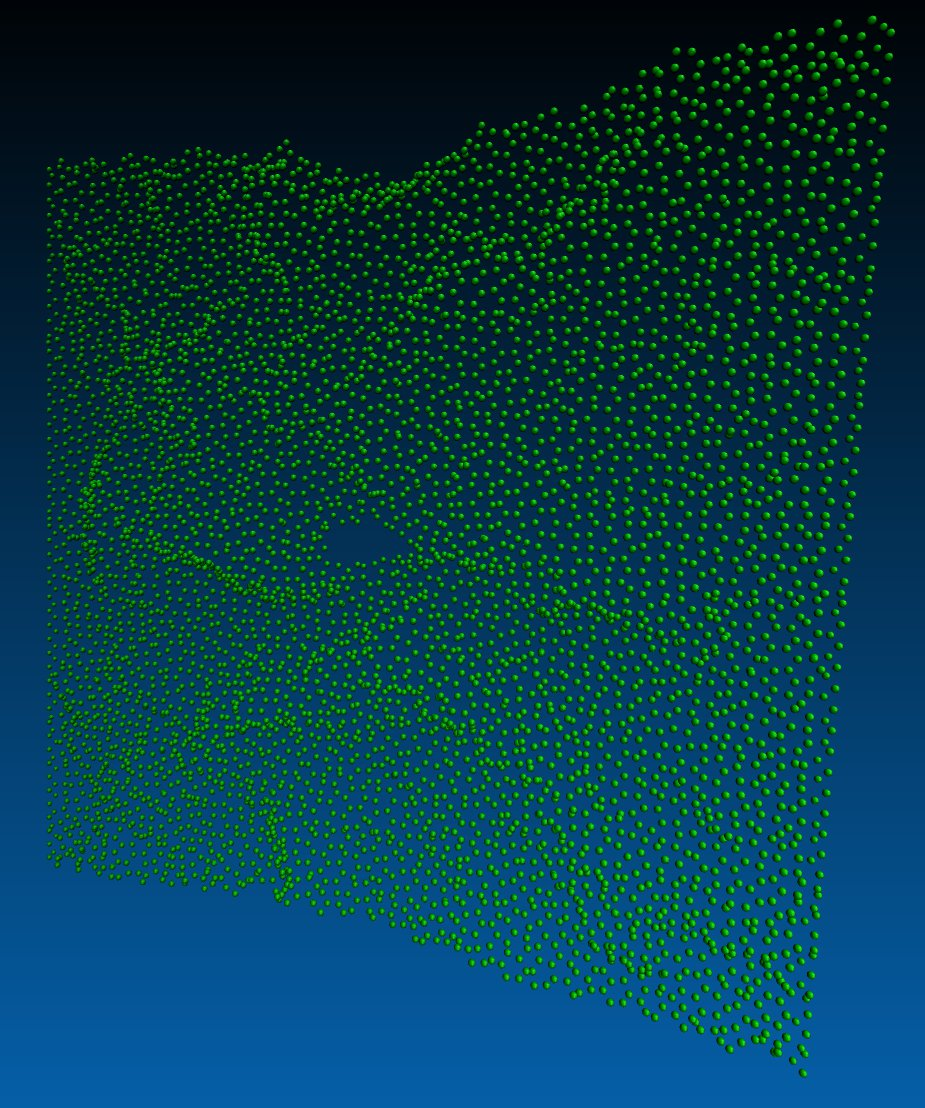
\includegraphics[width=0.5\textwidth]{snapmembranesouspression.jpg}
\begin{minipage}{0.5\linewidth}
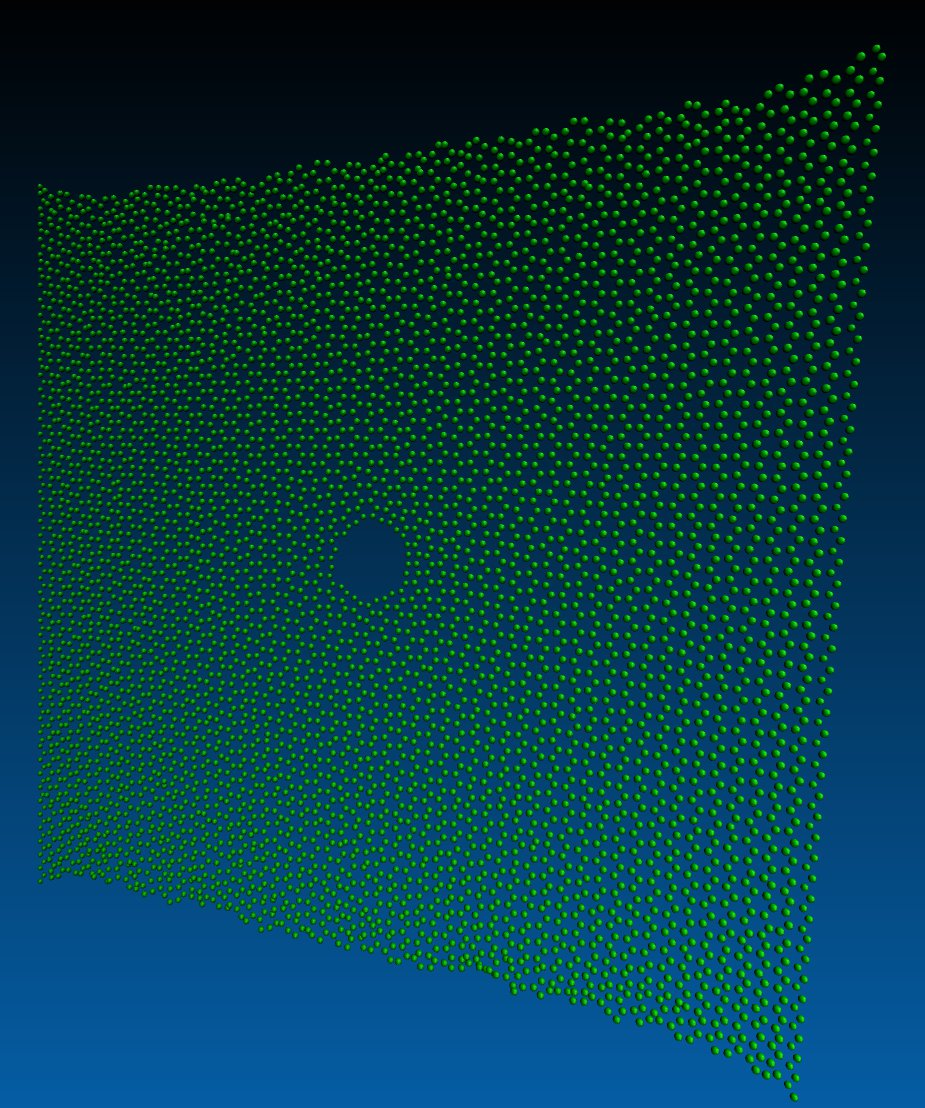
\includegraphics[width=1\textwidth]{snapmembranenontendue.jpg} 
\end{minipage}
\begin{minipage}{0.49\linewidth}
\caption[Tension au sein de la membrane]{La variation du facteur géométrique $lf$ permet, tout en conservant un nombre de grains et une taille de membrane constants de jouer sur la tension au sein de la membrane. Il est possible d'avoir des régimes dans lesquels la membrane est sous tension (image en haut à gauche), est sous pression (image en haut à droite), ou n'est ni tendu ni sous pression (image du bas).}
\label{snapshottensionmembranesnapshot}
\end{minipage}

\end{center}
\end{figure}



\newpage

\subsection{Membrane sous tension}

Pour commencer, interessons nous au cas d'une membrane fortement tendue, puor cela nous avons choisi un $lf=1.68$, ce qui nous situ dans le premier régime décri sur la figure \ref{tensionmembrane}. Il s'agit du régime pour lequel nous nous attendons à des résultats les plus proches du cas précédent. En effet la membrane étant sous tension, les déplacement perpendiculaires seront plus limités.



\begin{figure}[H]
\begin{center}
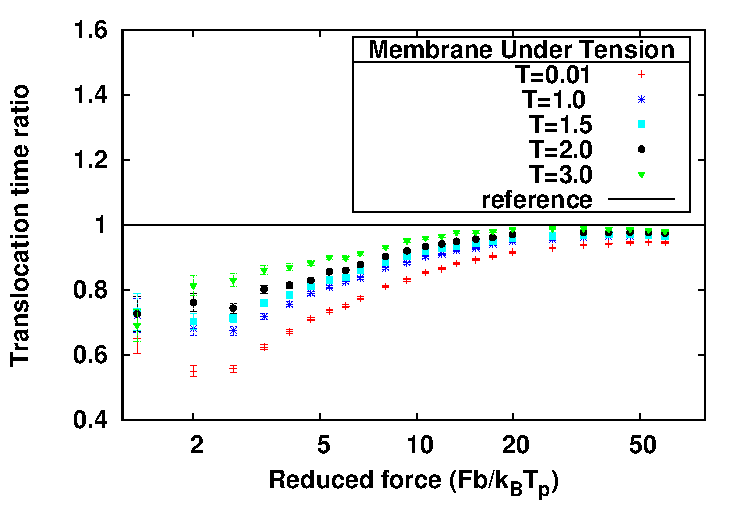
\includegraphics[width=1\textwidth]{hightension.pdf} 
\label{membranetendueevoltemp}
\end{center}
\end{figure}




\begin{figure}[H]
\begin{center}
\begin{minipage}{0.7\linewidth}
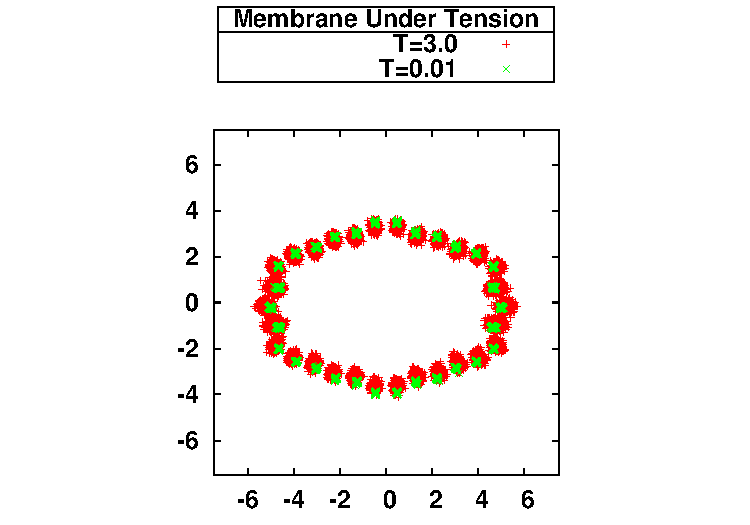
\includegraphics[width=1.2\textwidth]{2dhighmembranetension.pdf} 
\end{minipage}
\begin{minipage}{0.29\linewidth}
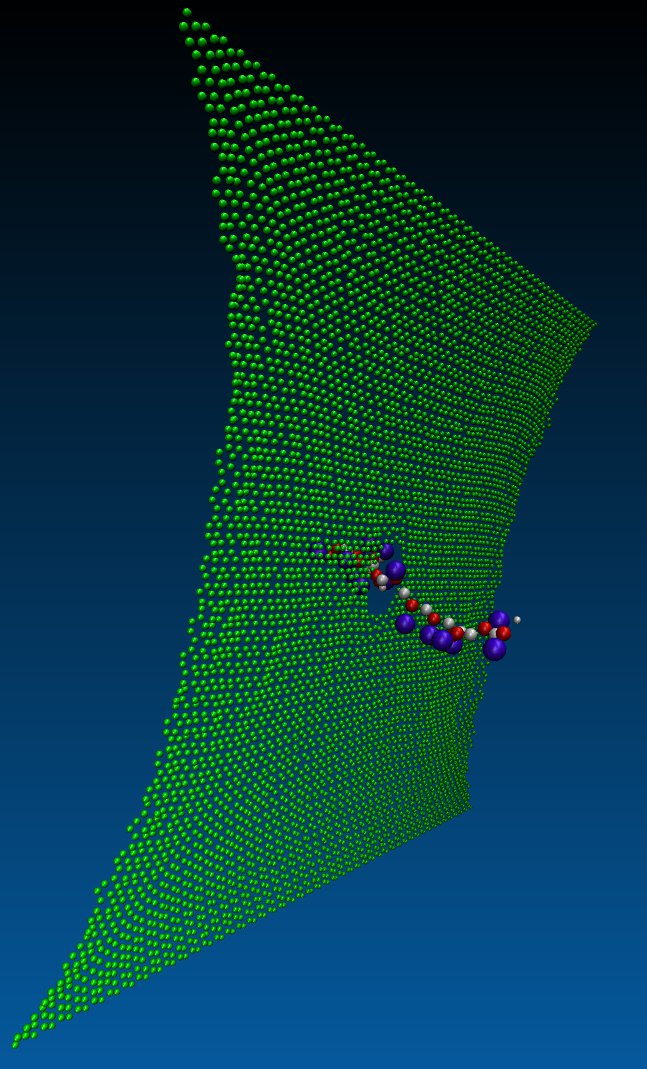
\includegraphics[width=1.1\textwidth]{membranetendue.jpg}
\end{minipage}
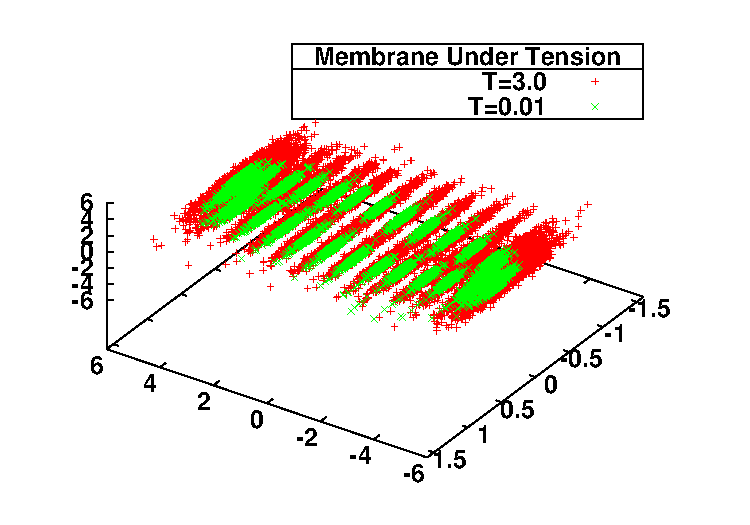
\includegraphics[width=\textwidth]{3dhighmembranetension.pdf}  
\caption[Membrane tendue]{bla}

\label{membranetendue}
\end{center}
\end{figure}



\subsection{Membrane non tendue}

$lf=1.81786$


\begin{figure}[H]
\begin{center}
\begin{minipage}{0.7\linewidth}
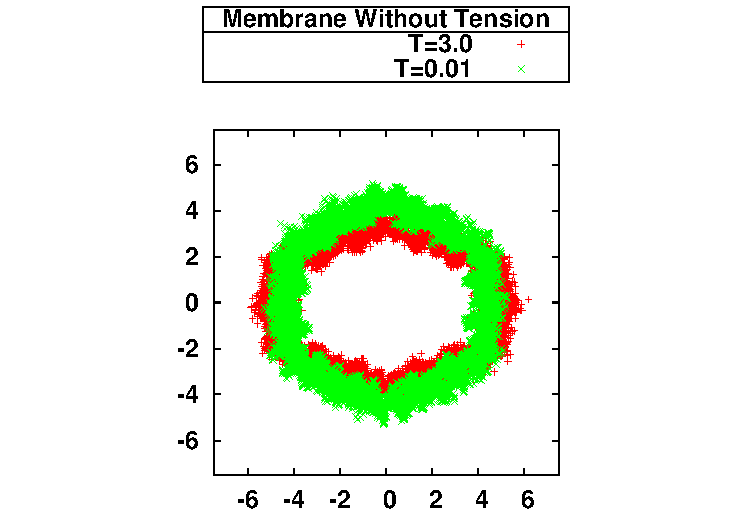
\includegraphics[width=1.2\textwidth]{2dnomembranetension.pdf} 
\end{minipage}
\begin{minipage}{0.29\linewidth}
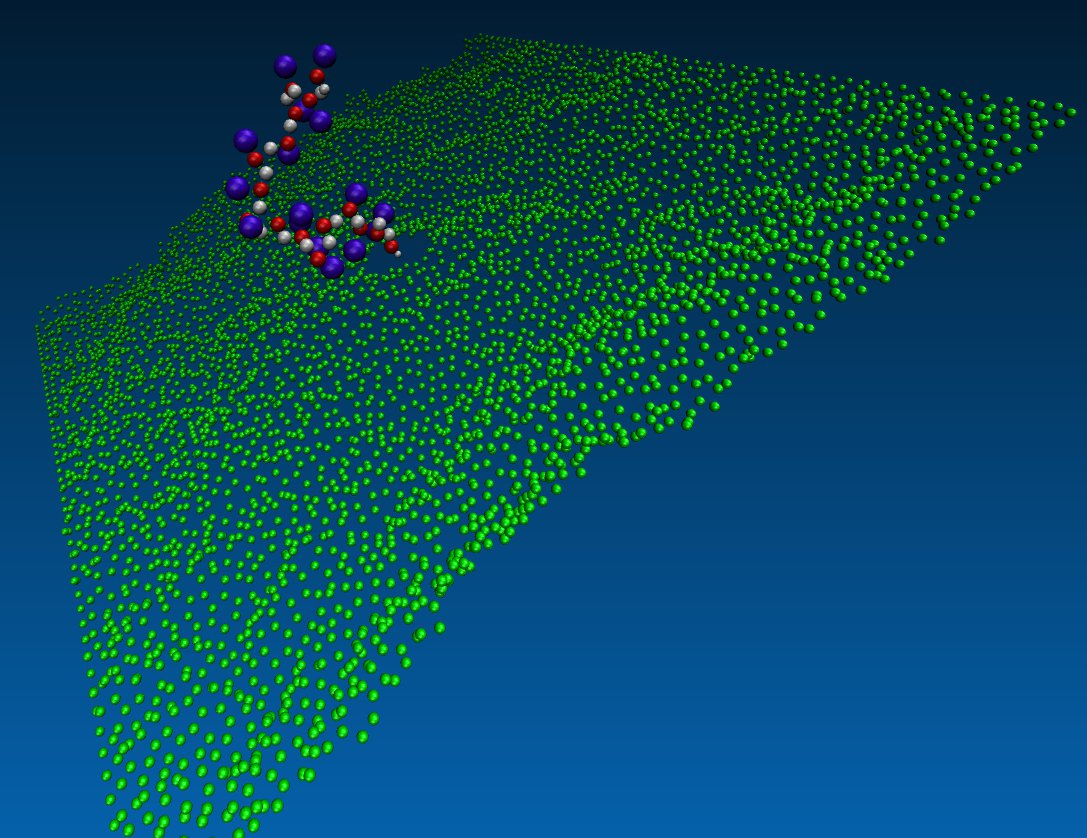
\includegraphics[width=1.1\textwidth]{membranenontendue.jpg}
\end{minipage}
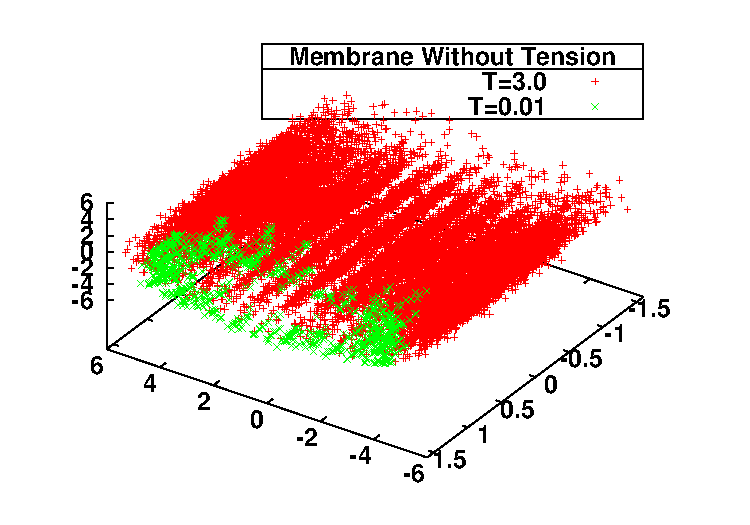
\includegraphics[width=\textwidth]{3dnomembranetension.pdf}  
\caption[Membrane non tendue]{membrane tendue.}

\label{membrane non tendue}
\end{center}
\end{figure}

\begin{figure}[H]
\begin{center}
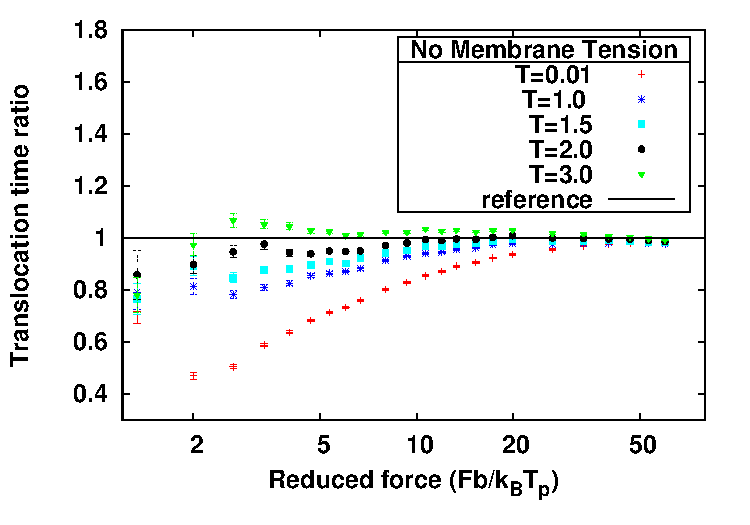
\includegraphics[width=1\textwidth]{notension.pdf} 
\label{membranenontendueevoltemp}
\end{center}
\end{figure}

\subsection{Membrane sous pression}

\begin{figure}[H]
\begin{center}
\begin{minipage}{0.7\linewidth}
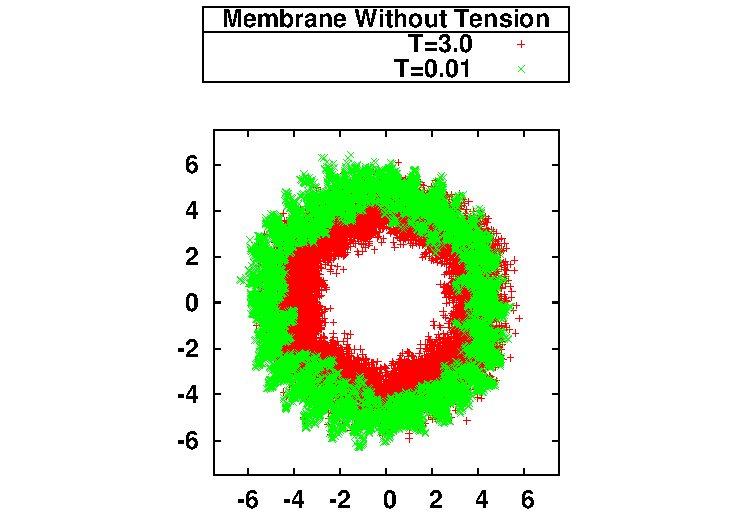
\includegraphics[width=1.2\textwidth]{2dmembranepressure.pdf} 
\end{minipage}
\begin{minipage}{0.29\linewidth}
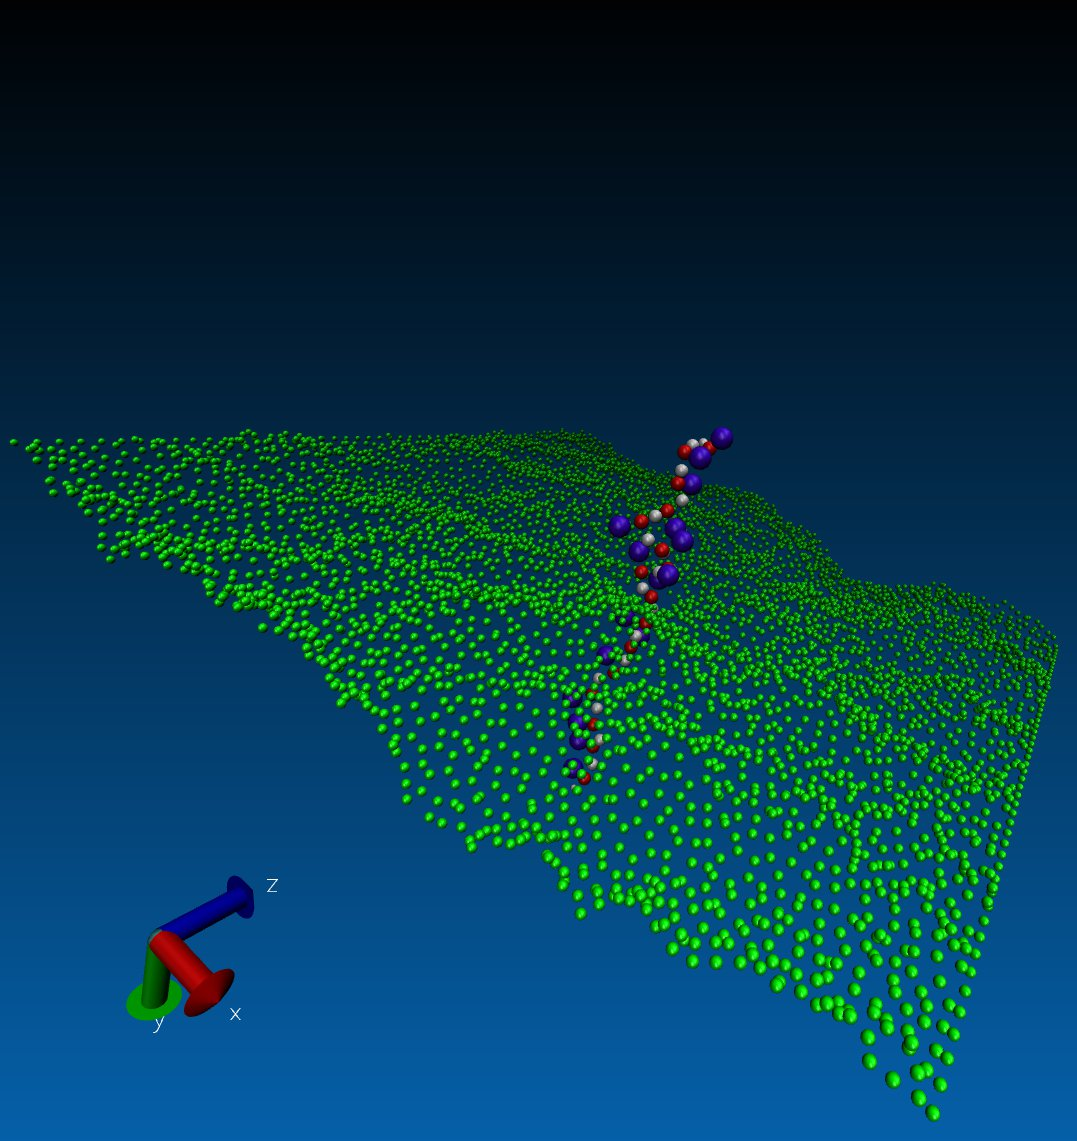
\includegraphics[width=1.1\textwidth]{membranesouspression.jpg}
\end{minipage}
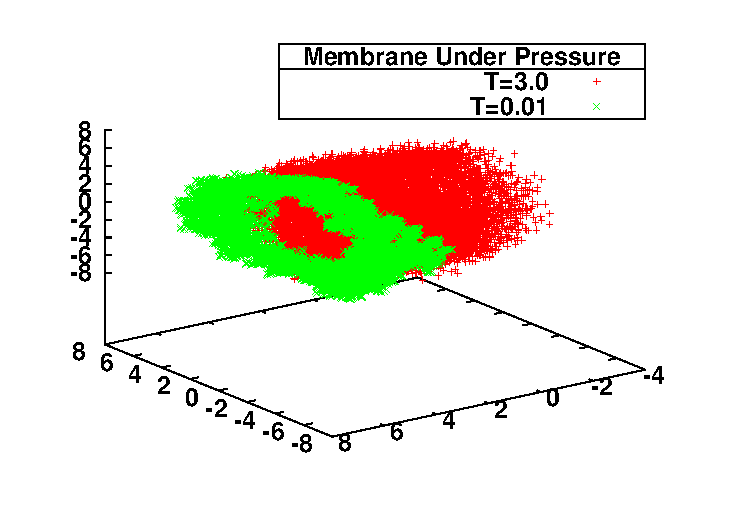
\includegraphics[width=\textwidth]{3dmembranepressure.pdf}  

\caption[Membrane sous pression]{membrane tendue.}
\label{reducedpore}
\end{center}
\end{figure}

\begin{figure}[H]
\begin{center}
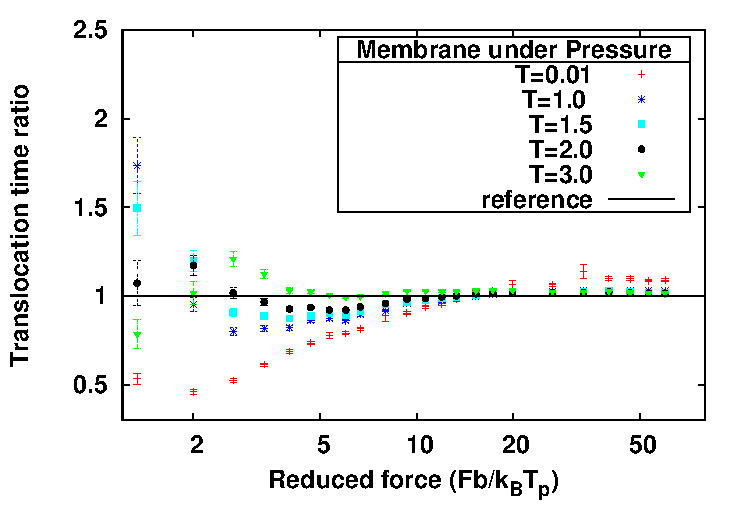
\includegraphics[width=1\textwidth]{lowtension.pdf} 
\label{membranepressionevoltemp}
\end{center}
\end{figure}


